\documentclass[12pt]{article}
\usepackage{amsmath,mathtools}
\usepackage[usenames,dvipsnames]{xcolor}
\usepackage[ngerman]{babel}
\usepackage[utf8]{inputenc}
\usepackage[T1]{fontenc}
\usepackage{libertine}
\usepackage{microtype}
\usepackage{fancyhdr}
\usepackage{sectsty}
\usepackage{setspace}
\usepackage{booktabs} % To thicken table lines
\usepackage[version=4]{mhchem}
\usepackage{tabularx}
\usepackage[ddmmyyyy]{datetime}
\renewcommand{\dateseparator}{.}
\usepackage{overcite}
\renewcommand\citeform[1]{[#1]}
\usepackage{siunitx}
\sisetup{detect-weight=true, detect-family=true}
\sisetup{text-celsius = $^\circ\mkern-1mu$C}
\sectionfont{\fontsize{12}{15}\selectfont}
\pagestyle{fancy}
\cfoot{\thepage}
\lhead{Nevroz Arslan }
\rhead{\today}
\setlength{\headheight}{15pt}
\renewcommand{\thesection}{\arabic{section}.}
\renewcommand{\thesubsection}{\thesection\arabic{subsection}}
\renewcommand{\headrulewidth}{0pt}
\renewcommand{\familydefault}{\sfdefault} 



\begin{document}
\begingroup
\leftskip=0cm plus 0.5fil \rightskip=0cm plus -0.5fil
\parfillskip=0cm plus 1fil
 \textbf{\large Darstellung von Ferrocenimin}\par
\endgroup

\begin{center}
 \textbf{Präparat Nr. 3 von 4}
\end{center}
\section{Reaktionstyp: \textnormal{Kondensation} }
\begin{figure}[ht]
\centering
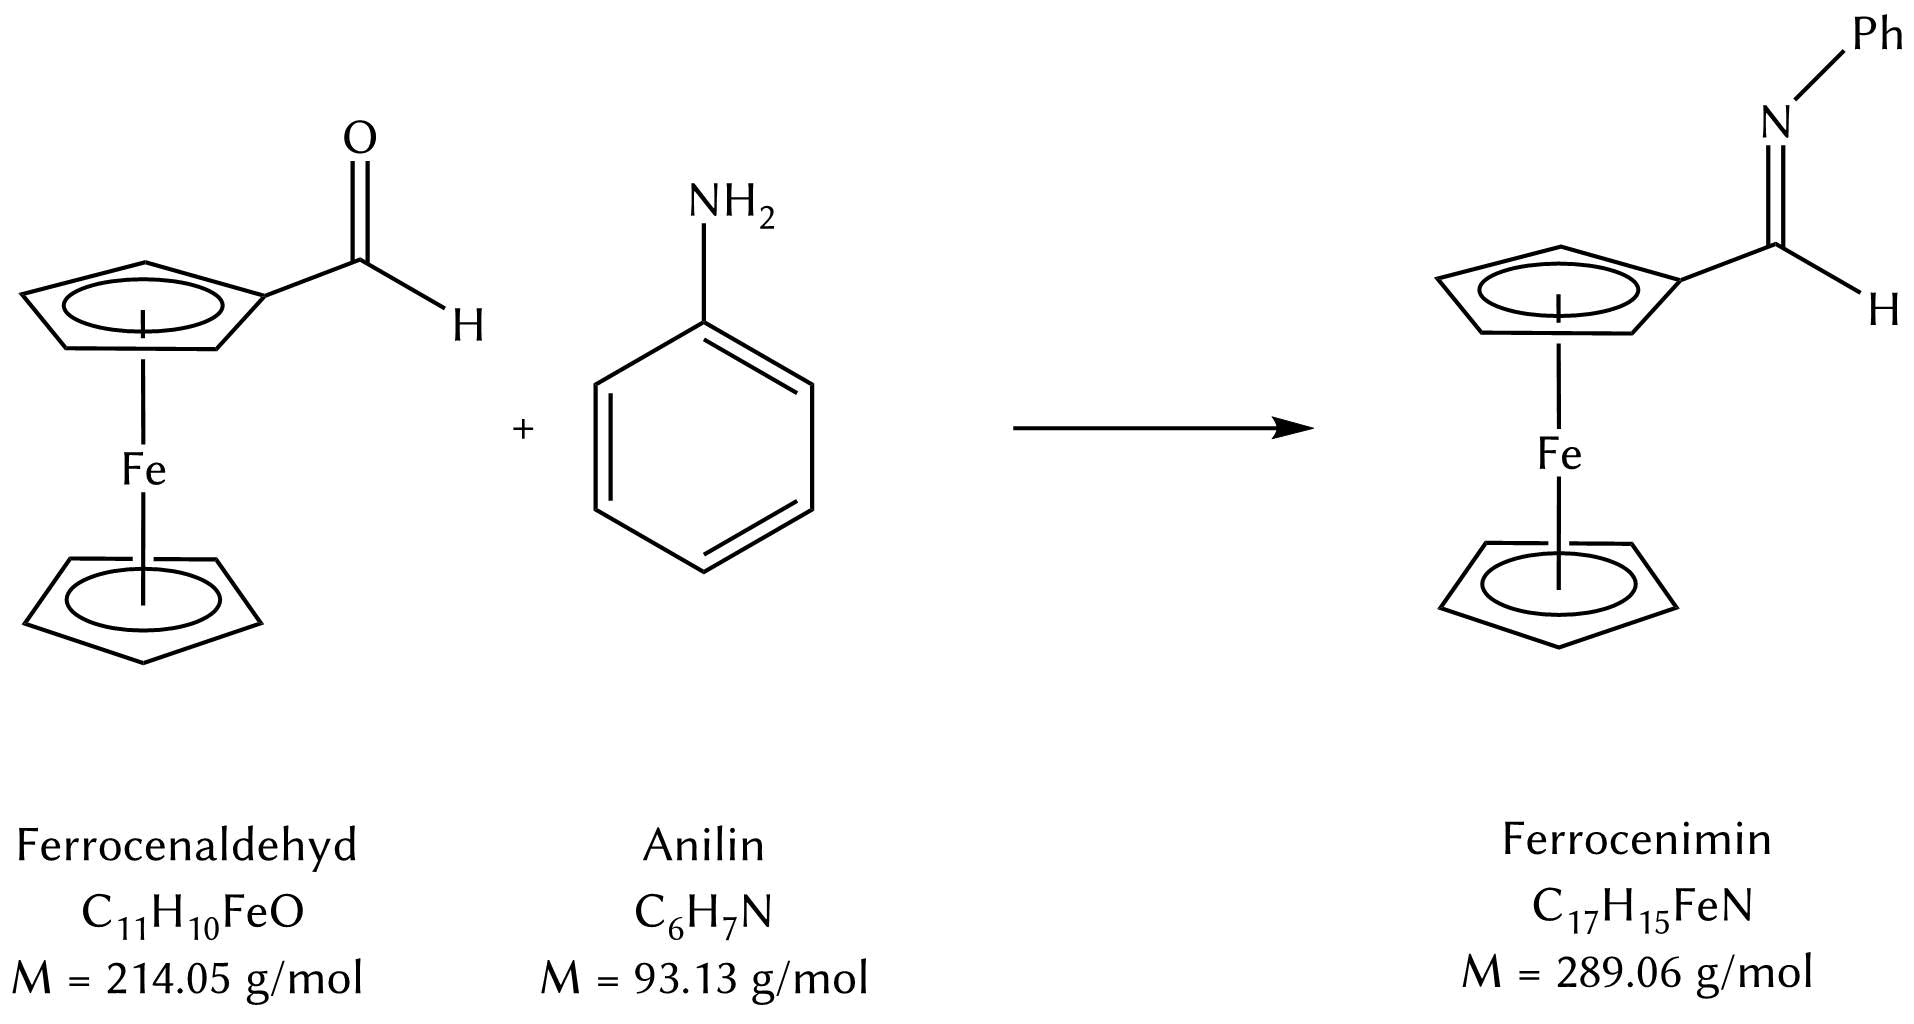
\includegraphics[width=\textwidth]{reaktion.png}
\end{figure}

\begin{onehalfspace}

\section{Berechnung des Ansatzes: }
Es sollte aus 0.312 g (1.46 \si{\milli\mol}) Ferrocenaldehyd Ferrocenphenylimin hergestellt werden.
Die Umrechnung des Literaturansatzes\cite{durch} ergab folgenden Ansatz:\\[0.5cm]
\begin{tabularx}{\textwidth}{lrrrr}
\toprule
\textbf{Bezeichnung}&\textbf{ M [\si{\gram\per\mol}]} & \textbf{n [\si{\milli\mol}]} & \textbf{Menge} & \textbf{Equiv}\\
\midrule
Ferrocenaldehyd & 214.04 & 1.46  &  0.312 \si{\gram} &1.00   \\
Anilin          & 93.13  & 1.46  &  0.13 \si{\milli\liter} & 1.00  \\
Diethylether    &  &  &  & LM   \\
\bottomrule
\end{tabularx}


\normalsize \section{Durchführung \cite{durch}}
In einem 250 \si{\milli\liter} Rundkolben, ausgestattet mit Rückflusskühler, wurde Ferrocenaldehyd (0.312 g, 1.46 \si{\milli\mol}) in Diethylether (20 \si{\milli\liter}) mit Molsieb 3 \si{\angstrom} vorgelegt und mit Anilin (0.13 \si{\milli\liter}, 1.46 \si{\milli\mol}) versetzt. Das Reaktionsgemisch wurde bei Raumtemperatur drei Stunden lang gerührt und anschließend filtriert. Das abgetrennte Molsieb wurde mit Diethylether gewaschen. Die vereinten Auszüge wurden am Rotationsverdampfer eingeengt und aus \textit{n}-Hexan umkristallisiert. Das Produkt (0.207 \si{\gram}, 0.72 \si{\milli\mol}, 3 \%) wurde als dunkelroter Feststoff erhalten.

\section{Ausbeute}
\begin{tabular}{ll}
  0.422 \si{\gram} (1.46 \si{\milli\mol}) =  & 100 \%\\
  0.207 \si{\gram} (0.72 \si{\milli\mol}) =  & 3 \%  \\
\end{tabular}
\section{Spektrenauswertung}
\begin{figure}[!ht]
   \centering
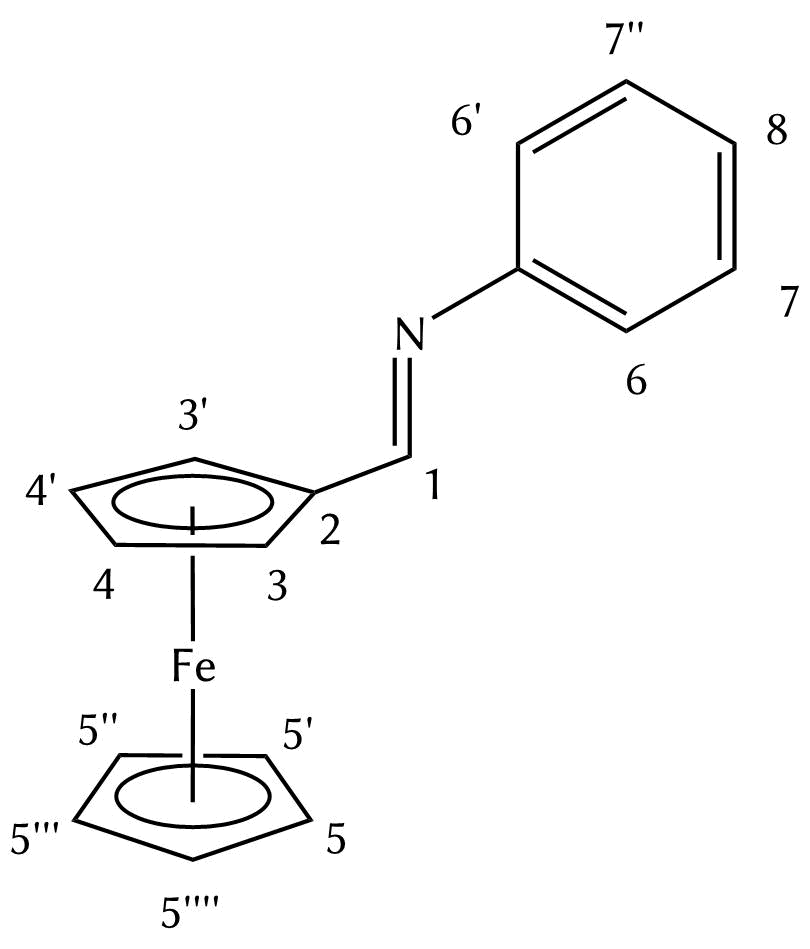
\includegraphics[scale=0.3]{auswert.png}
\end{figure}
\noindent
\textbf{\ce{^1_{}H-NMR}} (300 MHz, \ce{CDCl_3}): \ce{$\delta$} = 
4.22 (s, 5 H, 5-H),
4.55 (s, 2 H, 4-H),
4.73 (s, 2 H, 3-H),
7.03 - 7.36 (m, 5 H, 6-H, 7-H, 8-H),
9.92 (s, 1 H, 1-H) ppm.
\section{Mechanismus\cite{bio}}
Zunächst erfolgt ein nucleophiler Angriff des Anilins (\textbf{2}) am Carbonyl-C-
Atom des Ferrocenaldehyds (\textbf{1}). Hierbei bildet sich eine dipolare Zwischenstufe \textbf{3} 
und daraus ein geminaler Aminoalkohol \textbf{4}. Letztere Verbindung \textbf{4} wandelt sich durch Abspaltung
von Wasser in das gewünschte Produkt Ferrocenphenylimin (\textbf{5}) um.
\begin{figure}[!htbp]
   \centering
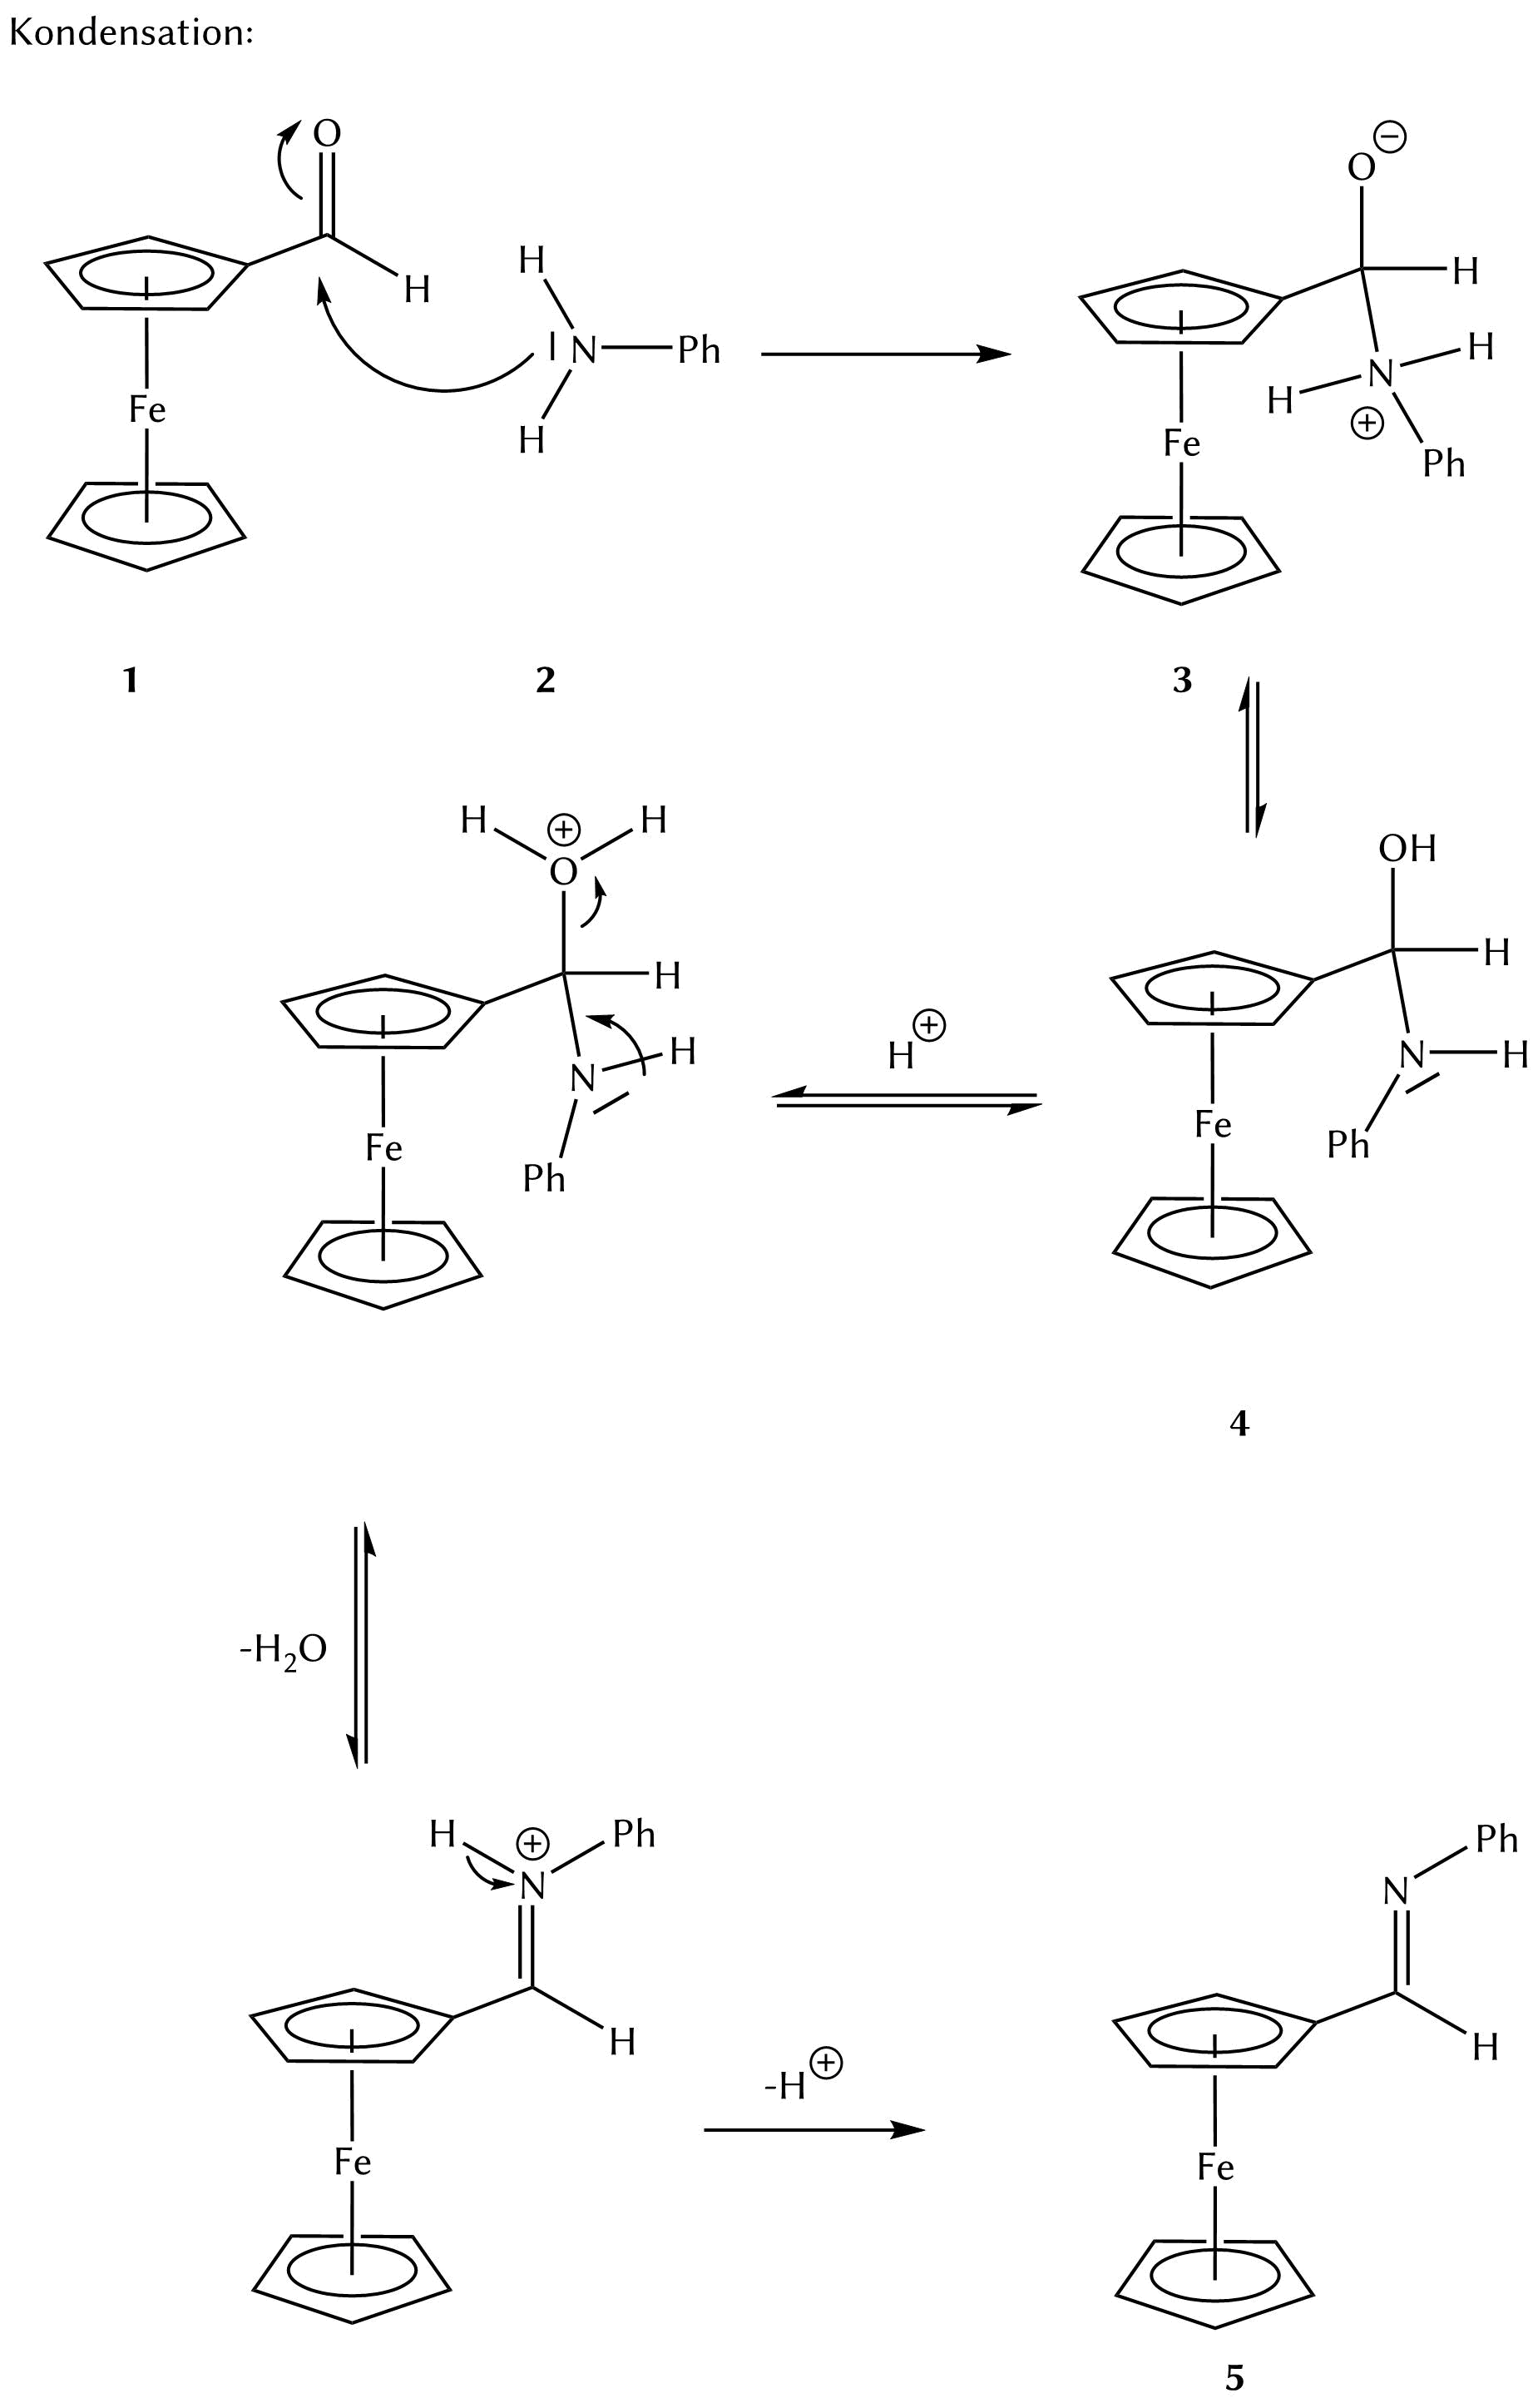
\includegraphics[scale=0.27]{mechan.png}
\end{figure}

\section{Abfallentsorgung}
Das im Rotationsverdampfer abgetrennte Lösungsmittel wurde im Behälter für halogenfreie Kohlenwasserstoffe entsorgt.
\section{Literatur}
\renewcommand{\section}[2]{}%
\begin{thebibliography}{}
%\bibitem{organikum}
%H. Becker \textit{Organikum}, 21. Aufl., Wiley-VCH, Weinheim \textbf{2009}, S. 528.
\bibitem{durch}
Hausvorschrift
\bibitem{bio}
J. Buddrus, \textit{Grundlagen der Organische Chemie}, 4. Aufl., De Gruyter, Berlin \textbf{2011}, S. 489.
\end{thebibliography}
\end{onehalfspace}
\end{document}